\subsection{Setup}
% ============================ FRAME 14 ==========================================>
\begin{frame}
	\frametitle{Setup}
	\begin{figure}
		\centering
		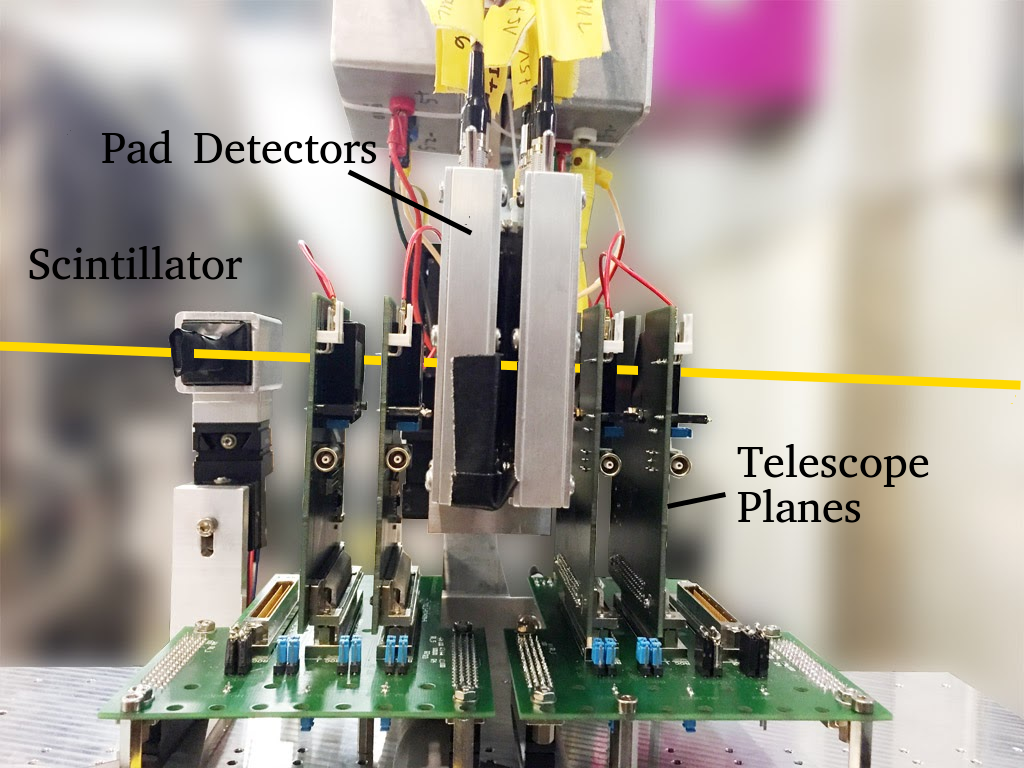
\includegraphics[width=5.5cm]{Setup}
	\end{figure}
	\begin{itemize}
		\setlength{\itemsep}{\fill}
		\item 4 tracking planes with analogue CMS pixel chips \ra provide scalable trigger
		\item 2 diamond pad detectors
		\item scintillator for precise trigger timing: sigma of \SI{1.3\pm.1}{ns}
		\item resolution: \SI{\sim80x50}{\micro\meter}
	\end{itemize}
\end{frame}
% ============================ FRAME 15 ==========================================>
\begin{frame}
	\frametitle{Schematics}
	\begin{figure}
		\centering
		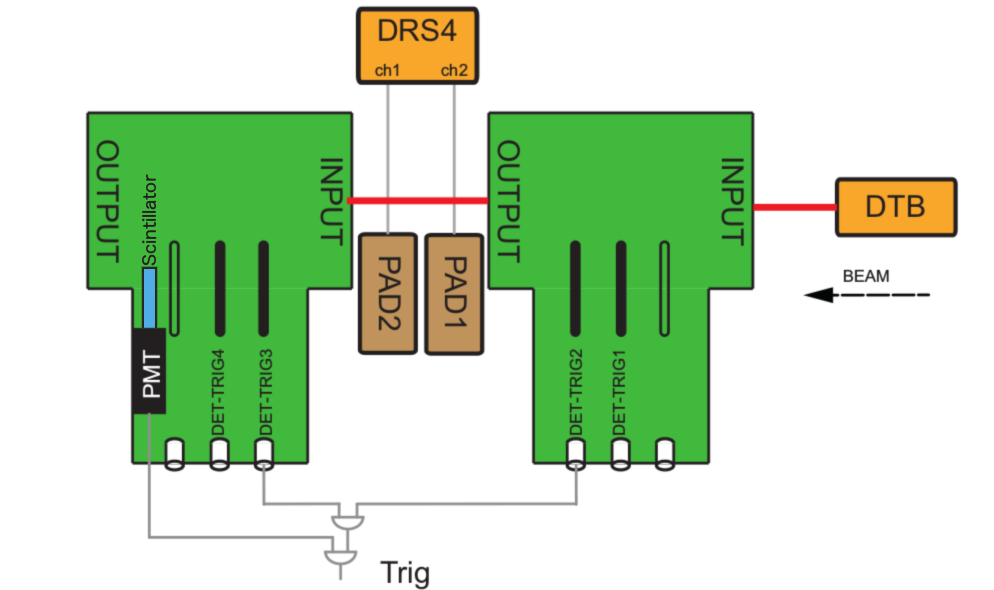
\includegraphics[width=7cm]{SchematicsV2}
	\end{figure}
	\begin{itemize}
		\setlength{\itemsep}{\fill}
		\item using PSI DRS4 Evaluation Board as digitizer for the pad waveforms
		\item using Digital Test Board (DTB) and pXar software for the telescope readout
		\item global trigger as coincidence of fastOR self trigger and scintillator signal
		\item EUDAQ as DAQ framework
	\end{itemize}
\end{frame}
% ============================ FRAME 16 ==========================================>
\begin{frame}
	\frametitle{DAQ}
	\begin{figure}
		\centering
		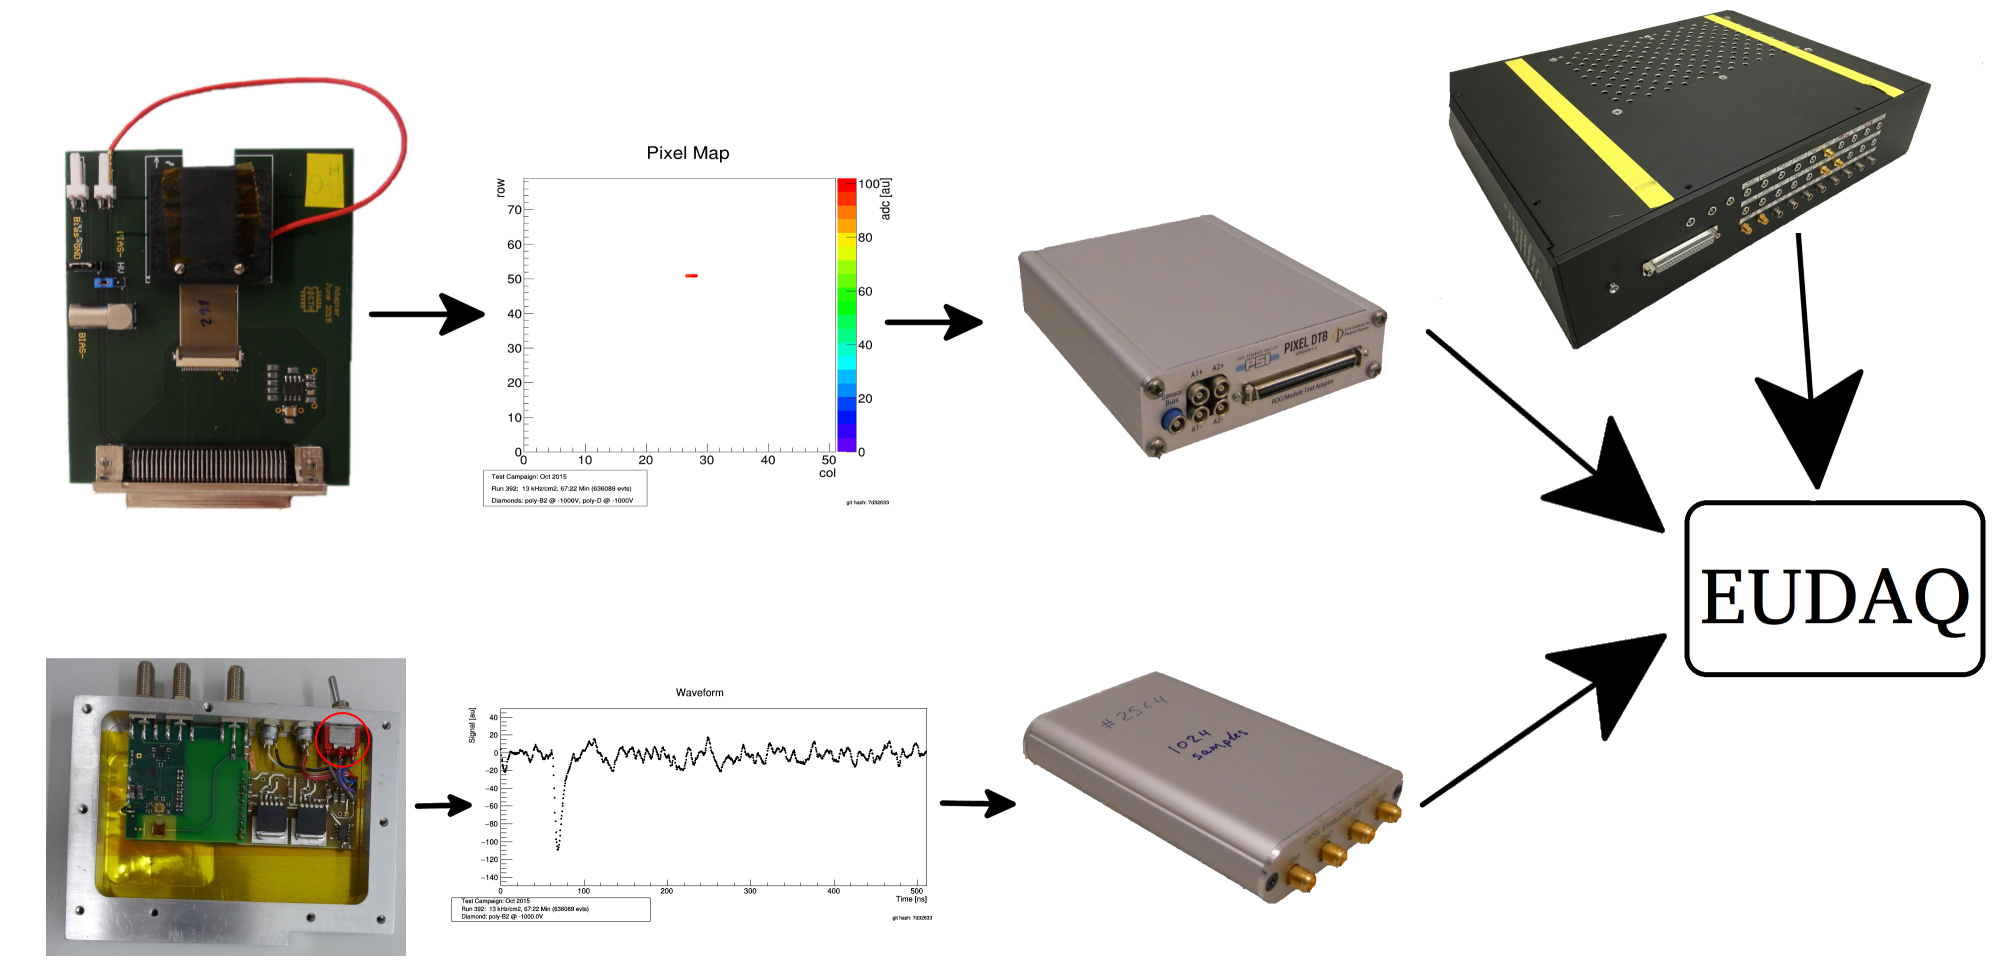
\includegraphics[width=.8\textwidth]{Intro}
	\end{figure}
	\begin{itemize}
		\item trigger unit to provide global trigger for all devices
		\item saving event based data stream as binary file using EUDAQ
	\end{itemize}
\end{frame}
% ============================ FRAME 17 ==========================================>
\begin{frame}
	\frametitle{Trigger Logic}
	\begin{minipage}[c][.5\textheight]{4cm}
		\begin{itemize}
			\setlength{\itemsep}{\fill}
			\item complicated trigger logic
			\item long setup time
			\item error prone
			\item varying cable length
		\end{itemize}
	\end{minipage}
	\begin{minipage}{8cm}
		\begin{figure}
			\centering
			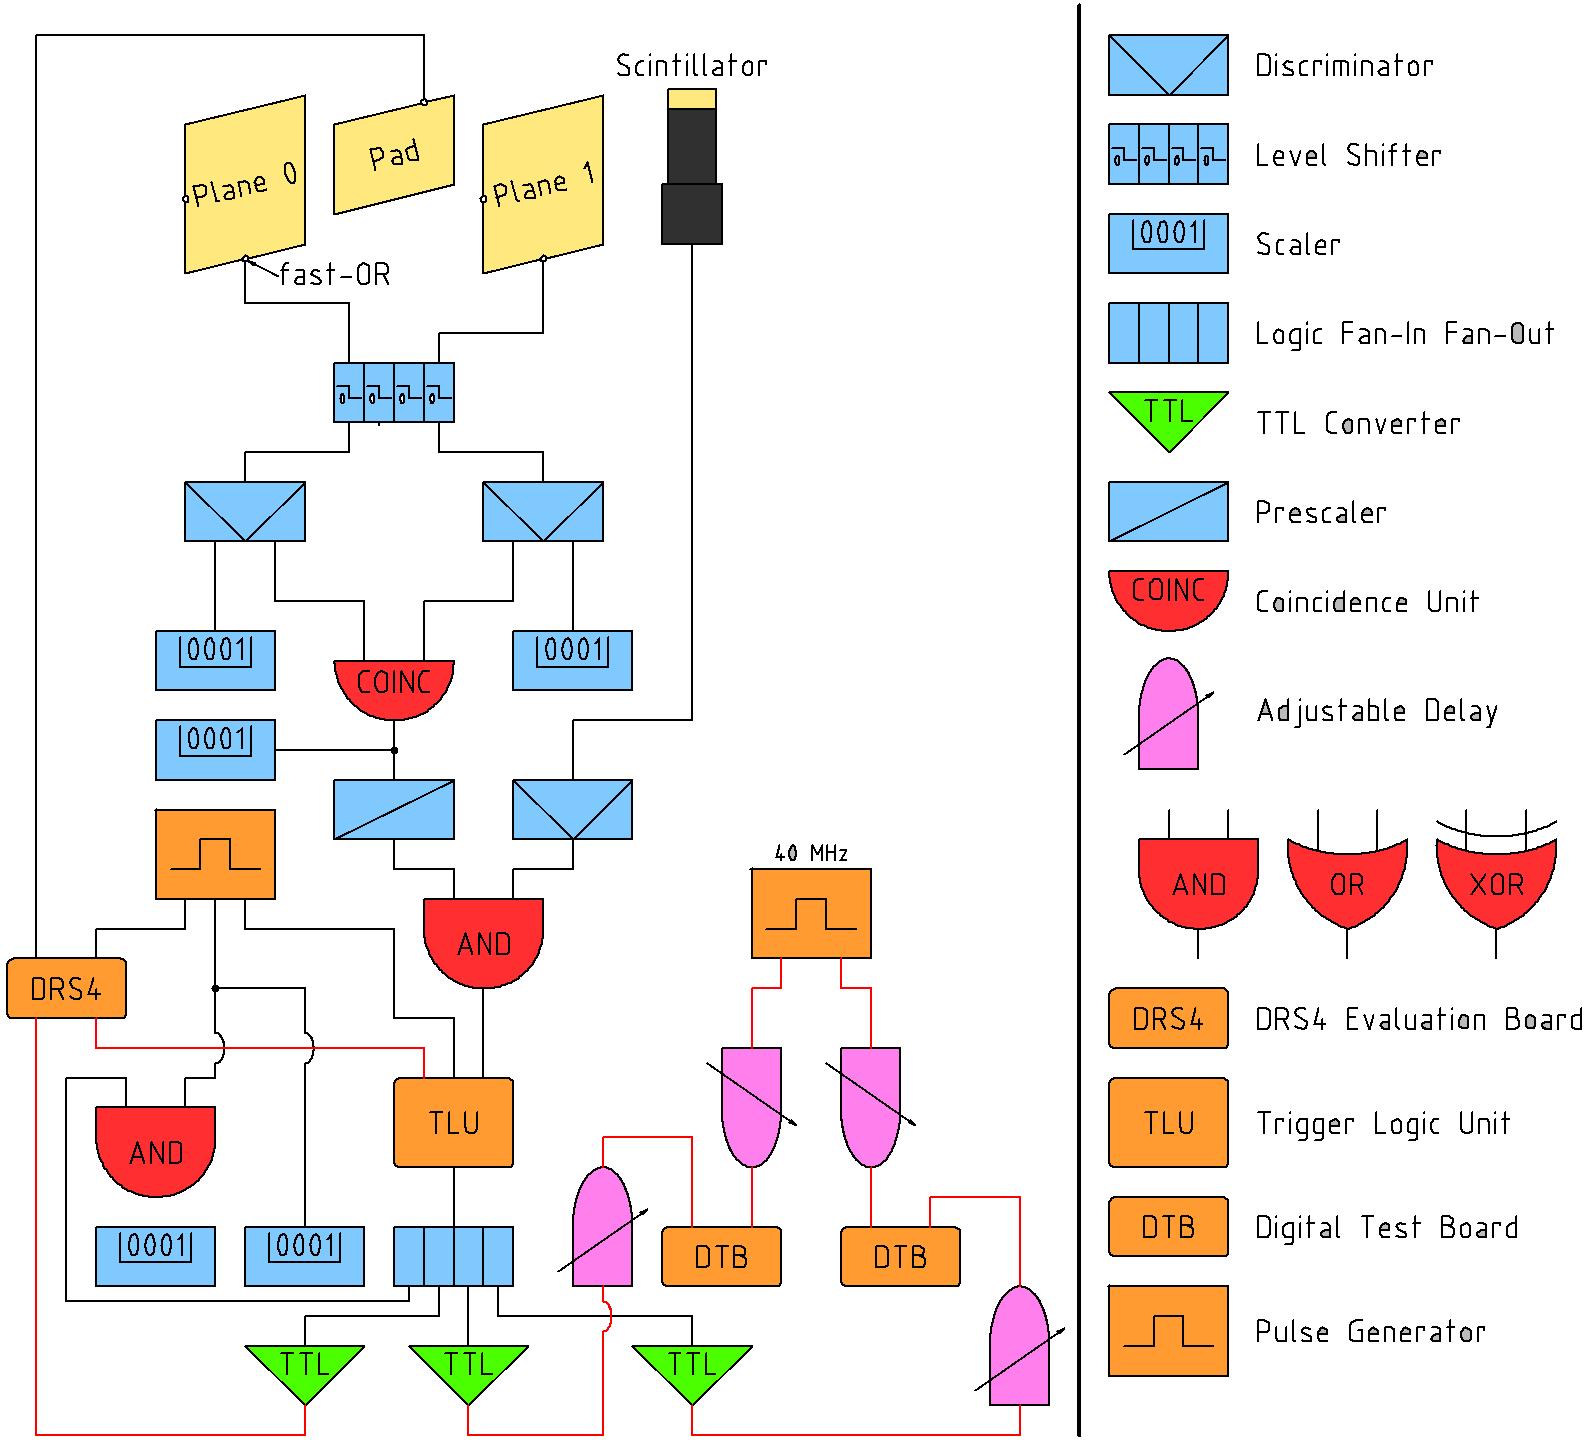
\includegraphics[width=7cm]{TrigLog}
		\end{figure}
	\end{minipage}
\end{frame}
% ============================ FRAME 18 ==========================================>
\begin{frame}
	\frametitle{Trigger unit (TU)}
	\begin{figure}
		\centering
		\begin{subfigure}[t]{0.2\textwidth}
			\centering
			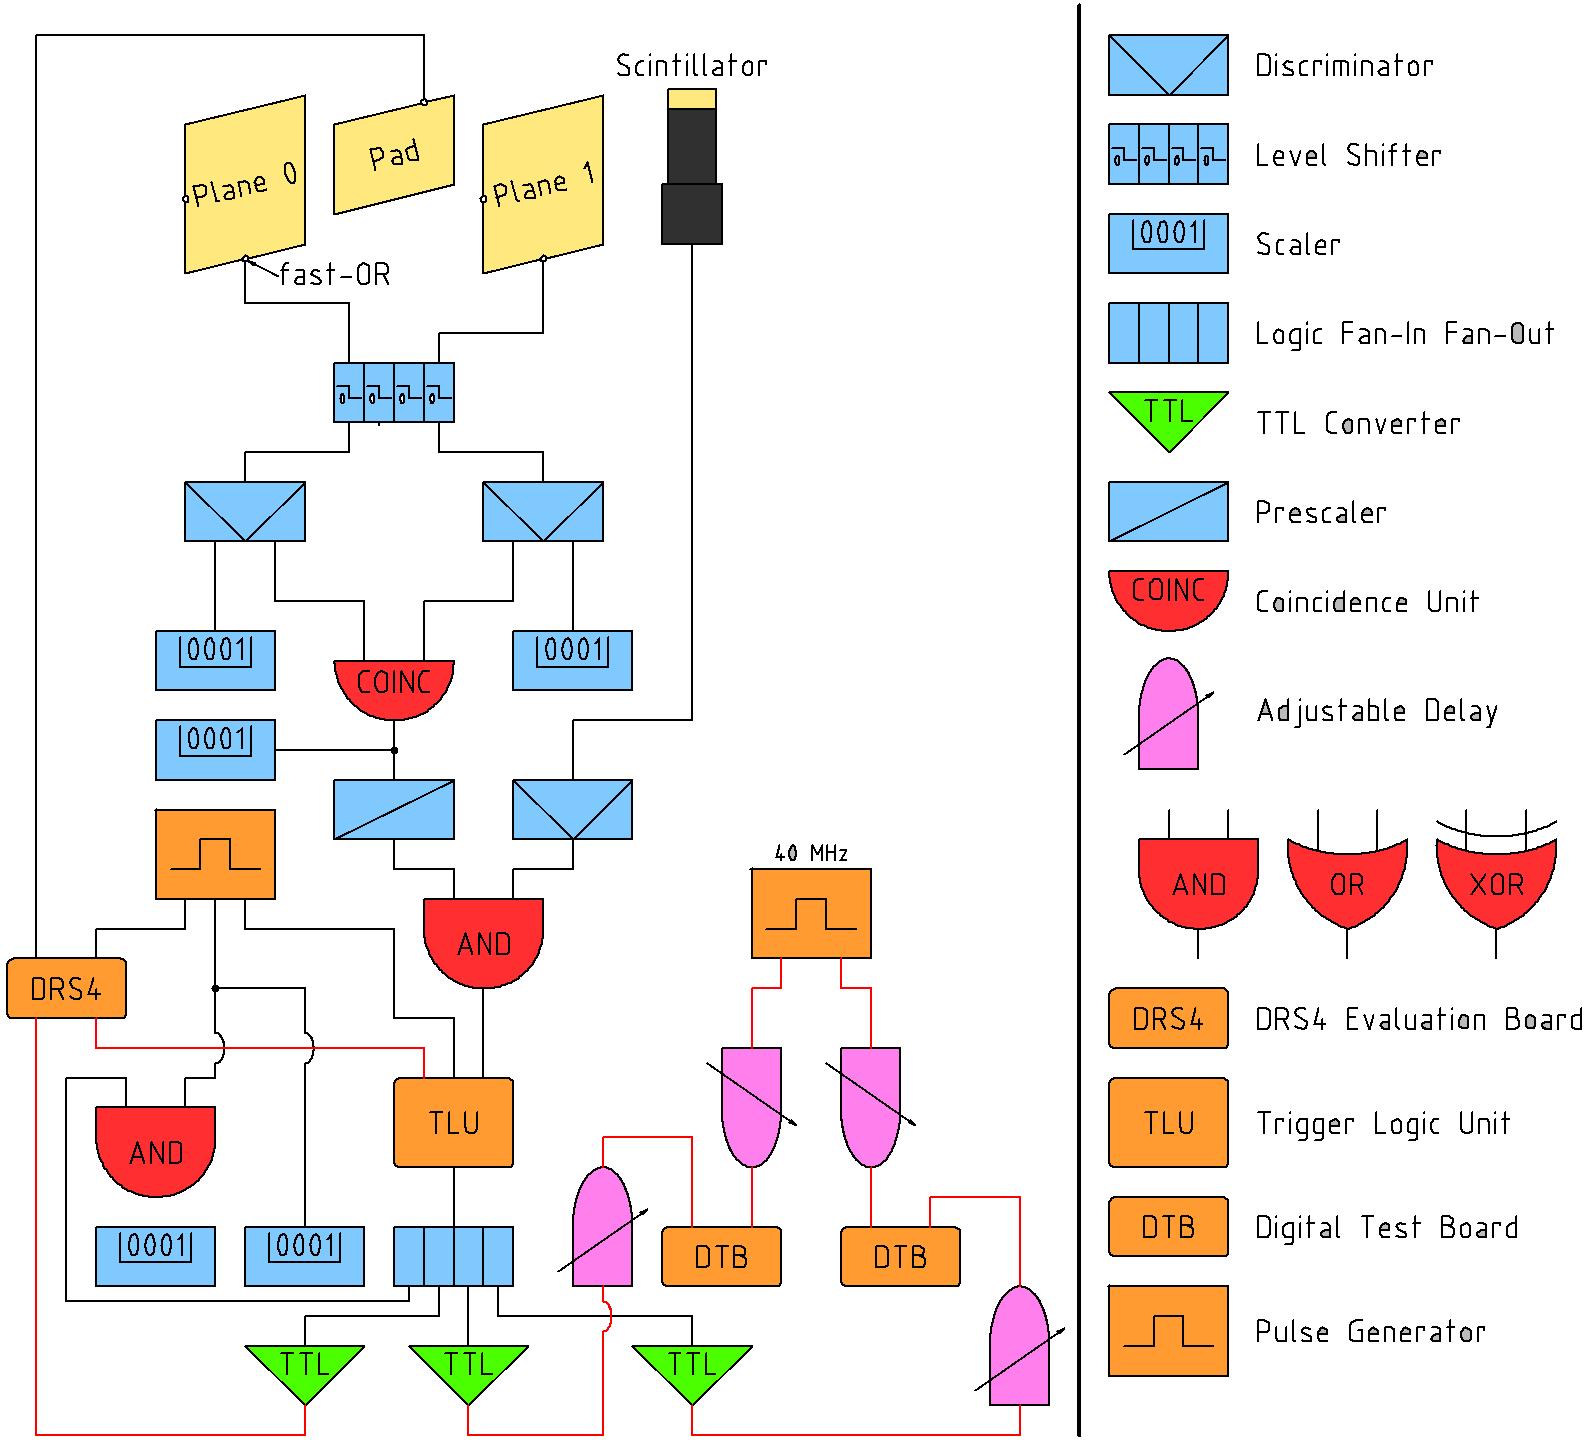
\includegraphics[height=2cm]{TrigLog}
		\end{subfigure}
		\ra
		\begin{subfigure}[t]{0.7\textwidth}
			\centering
			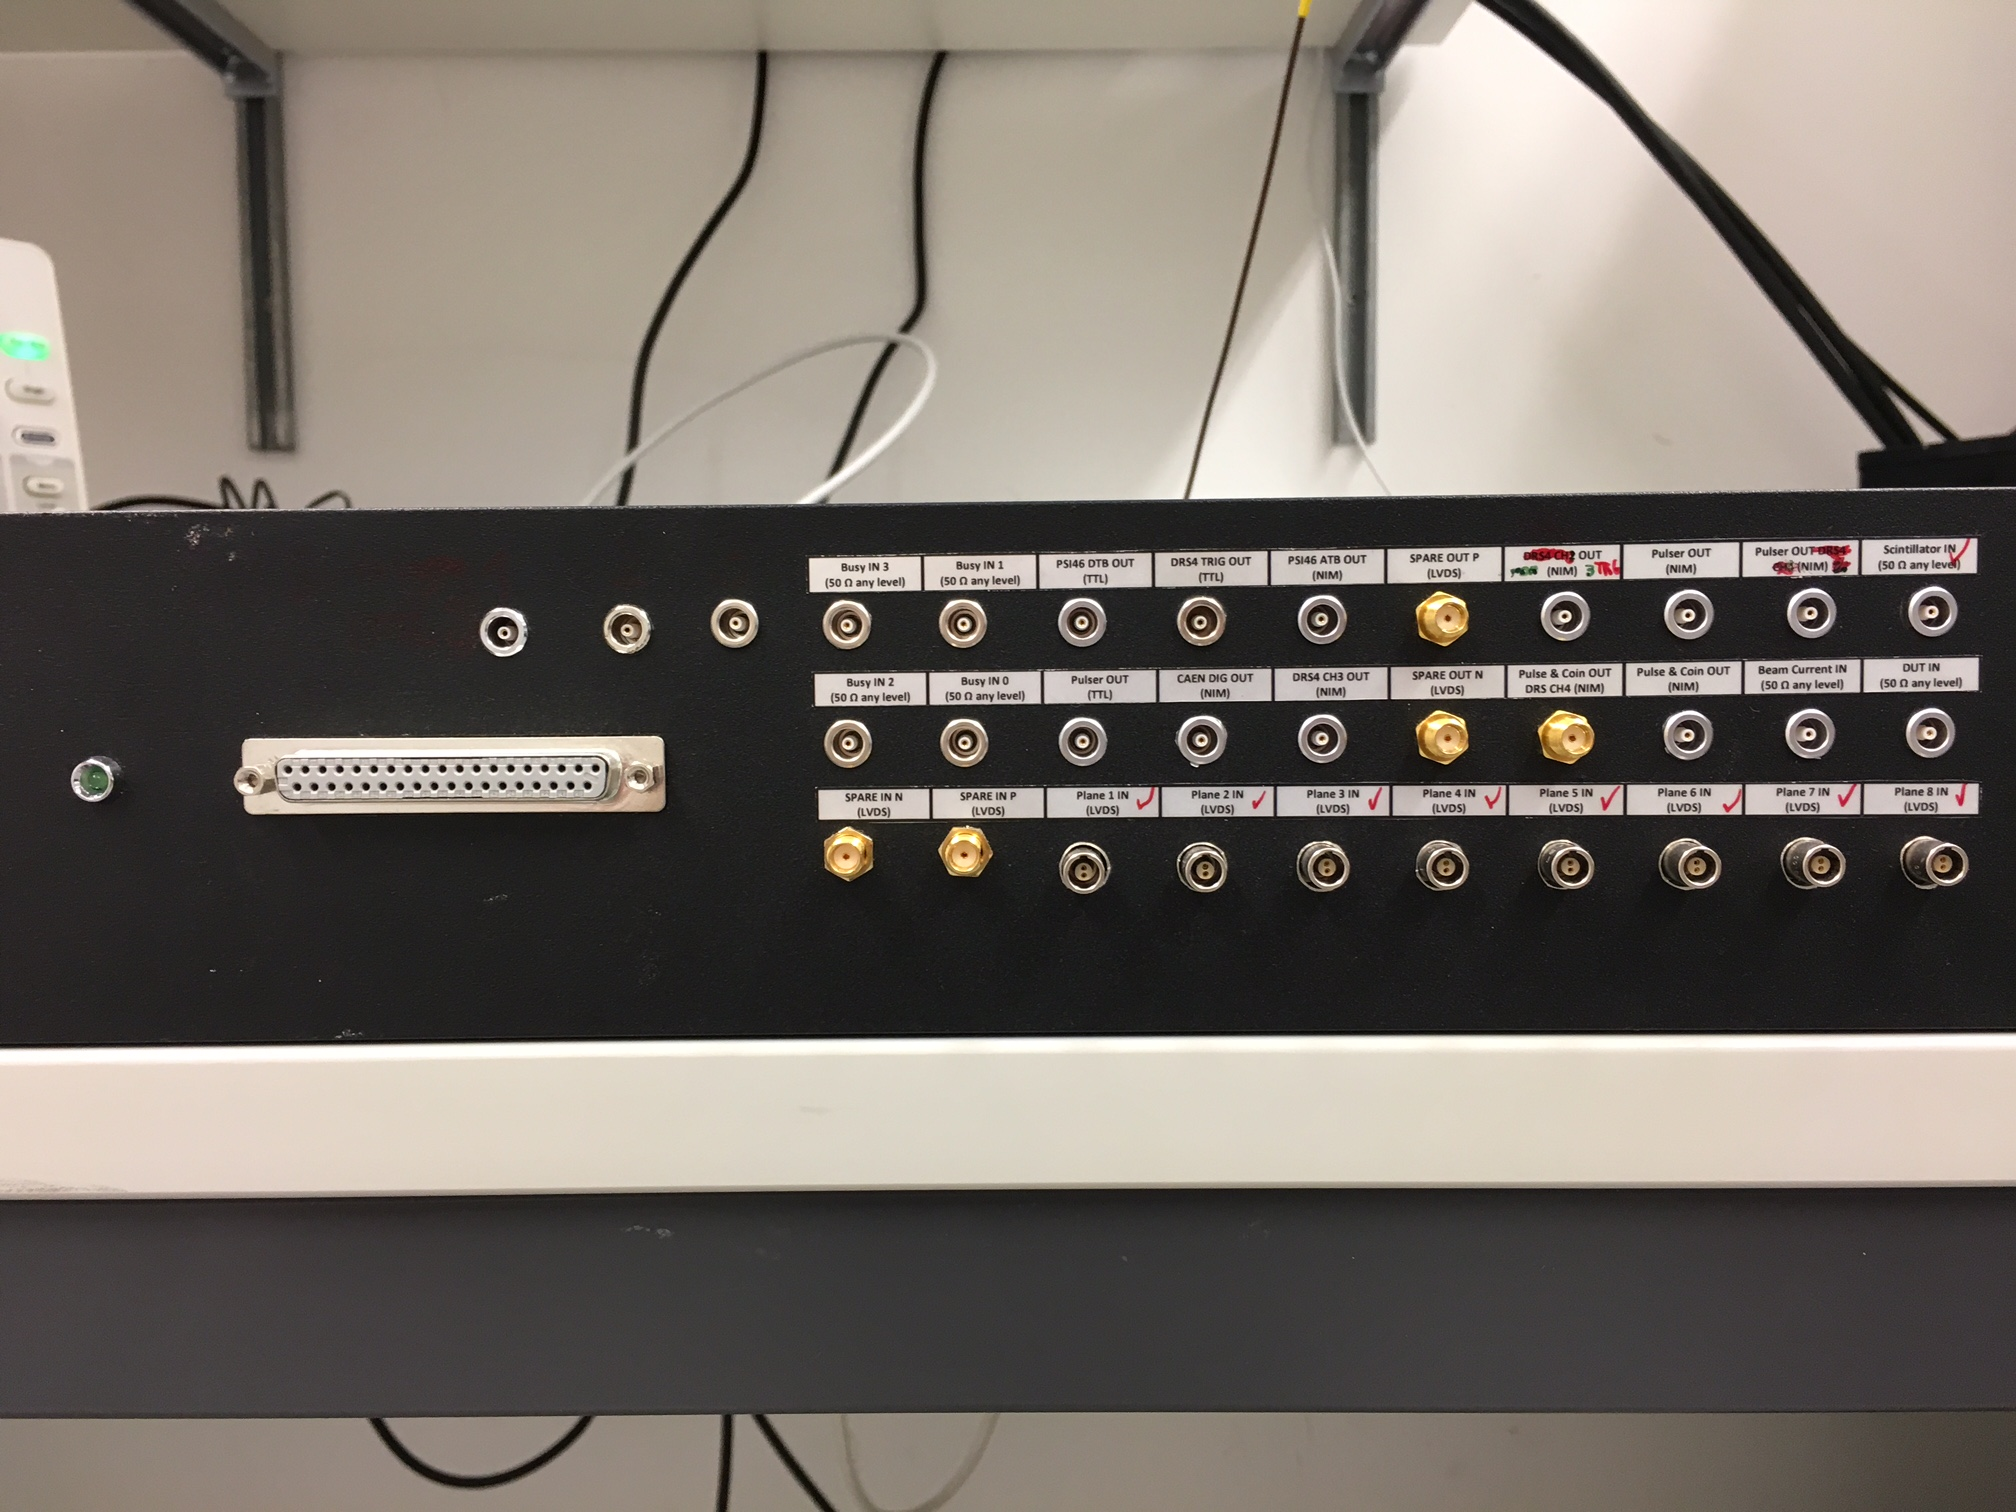
\includegraphics[height=2cm]{tu}
		\end{subfigure}
	\end{figure}
	\begin{itemize}
		\setlength{\itemsep}{\fill}
		\item handles (almost) all trigger logic of the setup with FPGA system
		\item provides scalers (counter) for the input triggers, pad signals and beam current
		\item sends calibration pulses as reference signal
		\item pre-scalers to guarantee stable pulser rates
		\item coincidence and handshake logic
	\end{itemize}
\end{frame}